%%%%%%%%%%%%%%%%%%%%%%%%%%%%
%\subsection{Validation of Calibration Hardware Systems}

All calibration designs presented in the previous section require full system validation before being deployed in the \dword{dune} \dword{fd}. Here, we describe the validation of a complete baseline design and some of the alternative designs described in the Appendix, Section~\ref{appx:calibration}.

Although laser calibration systems are being operated in other \dword{lartpc} experiments (e.g., \dword{microboone}, future \dword{sbnd} runs), they have stringent requirements in terms of mechanical and optical precision , long-term reliability, laser track length, performance of the \dword{lbls}, \dword{daq} interface, and effect on \efield, especially due to the \dword{fc} penetration. 
%with alternative design options
All of these lead to corresponding goals for a test installation and operation in \dword{pdsp} that could be done in the post-LS2 run. As Figure~\ref{fig:protoDUNESP_topView_marked} shows, \dword{pdsp} has ports of the same size as the \dword{dune} \dword{fd} that could be used for these tests. If a pair of ports can be used, then one could even have crossing tracks within a single drift volume. If one of the ports external to the \dword{tpc} can be used, then we would test the double-rotary alternative system described in Section~\ref{sec:sp-calib-laser-alter} and aimed at improving the coverage from the end-wall locations.

\begin{dunefigure}[Top view of the \dshort{pdsp} cryostat showing various penetrations]{fig:protoDUNESP_topView_marked}
{Top view of the \dword{pdsp} cryostat showing various penetrations. Ports marked in red are free and could be used to test the calibration systems. The four largest ports have the same diameter (\SI{250}{\milli\m}) as the calibration ports of DUNE \dword{fd}, and are located over the \dword{tpc}. The largest ports at the right side corners of the cryostat are the human access ports.}
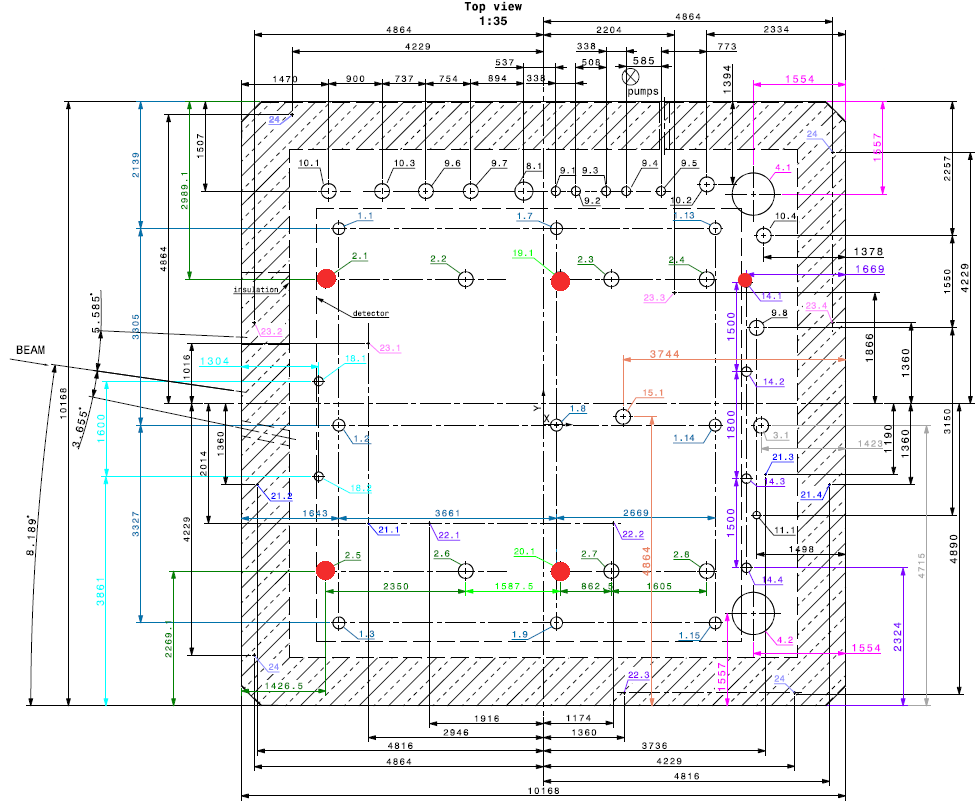
\includegraphics[height=4.0in]{protoDUNESP_topView_marked.png}
\end{dunefigure}

The goal for validation would be to test all aspects of the system design, installation, alignment, operation, interfaces with \dword{daq}, and analysis, among others. \dword{pdsp}, because it is located at the surface, could measure the \efield map with cosmic rays to compare with the one from the laser system to improve the analysis methods or identify weak aspects in the design. An important design parameter is the length of a laser track. Our design assumes that \SI{20}{\m} is possible. \dword{microboone} has demonstrated only up to \SI{10}{\m}, but the track could be longer, depending on laser intensity. Measurements are limited by the size of the detector, but one way to gain information on longer tracks is to make a scan with low laser intensities, so that the end of the track is  visible, and register how the maximum obtained track length scales with intensity. An extrapolation to the \dword{dune} \dword{fd} laser intensity would tell us the maximum length possible. Such a measurement could also be done at \dword{microboone} or \dword{sbnd}.

An important aspect of the development plan, to be carried out at \dword{pdsp2}, is the characterization of the charge created by the laser beam ionization as a function of distance travelled in the \dword{lar} and the laser beam intensity. This dependence is thought to be affected by self-focusing effects due to the high light intensity, but it can be studied by measuring the collected charge distribution from a series of tracks close, and parallel, to the \dword{apa}s in order to break any correlations with the electron lifetime. This measured charge function could then be used with tracks in different directions to obtain a measurement of electron lifetime, which would significantly increase the capabilities of the laser system. 

The pulsed neutron source is a new idea never used in other experiments, so a \dword{pdsp2} test is essential. The corner human access ports similar to the ones in the \dword{dune} \dword{fd} could be used for this test.


In addition to dedicated hardware validation runs at \dword{pdsp2}, other \dword{lar} experiments provide ample opportunities to develop and validate calibration tools and techniques, especially those relevant to the hardware being deployed. For example, the \dword{microboone} experiment is currently leading the development of analysis methods using laser data to extract an \efield map. Energy calibration techniques and related software tools are also being developed at various experiments (\dword{microboone}, ICARUS, \dword{lariat}, \dword{protodune}) that involve estimating and propagating uncertainties like \efield distortions, recombination, and other effects into physics signals. Other calibration related developments include \dword{daq} and calibration database design, all of which are being improved at \dword{sbn} and \dword{protodune}.
 
